% lintrans - The linear transformation visualizer
% Copyright (C) 2021-2022 D. Dyson (DoctorDalek1963)

% This program is licensed under GNU GPLv3, available here:
% <https://www.gnu.org/licenses/gpl-3.0.html>

\documentclass[../main.tex]{subfiles}

\begin{document}

\subsection{Evaluating success criteria\label{evaluation:evaluating-success-criteria}}

In \S\ref{analysis:success-criteria}, I laid out the success criteria for the project. It is now time to evaluate how well I met these criteria.

\subsubsection{Defining multiple matrices\label{evaluation:evaluating-success-criteria:define-multiple-matrices}}

Criterion~\ref{success-criterion:define-multiple-matrices} says that the user must be able to define matrices in at least two different ways. I have been using these dialogs during development and they're quite useful. I would say I have completely fulfilled this criterion.

\begin{figure}[H]
	\centering
	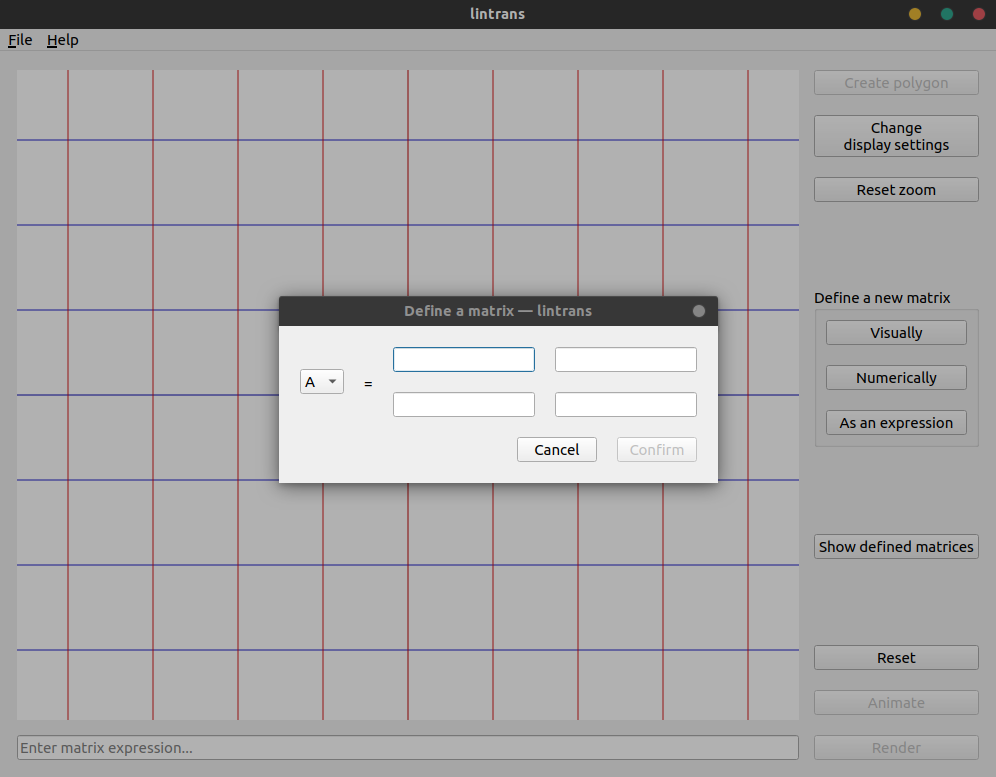
\includegraphics[width=0.95\linewidth]{evaluation/success-criteria/define-multiple-matrices/numerical-dialog.png}
	\caption{The numerical definition dialog}
	\label{fig:evaluation:success-criteria:define-multiple-matrices:numerical-dialog.png}
\end{figure}
\begin{figure}[H]
	\centering
	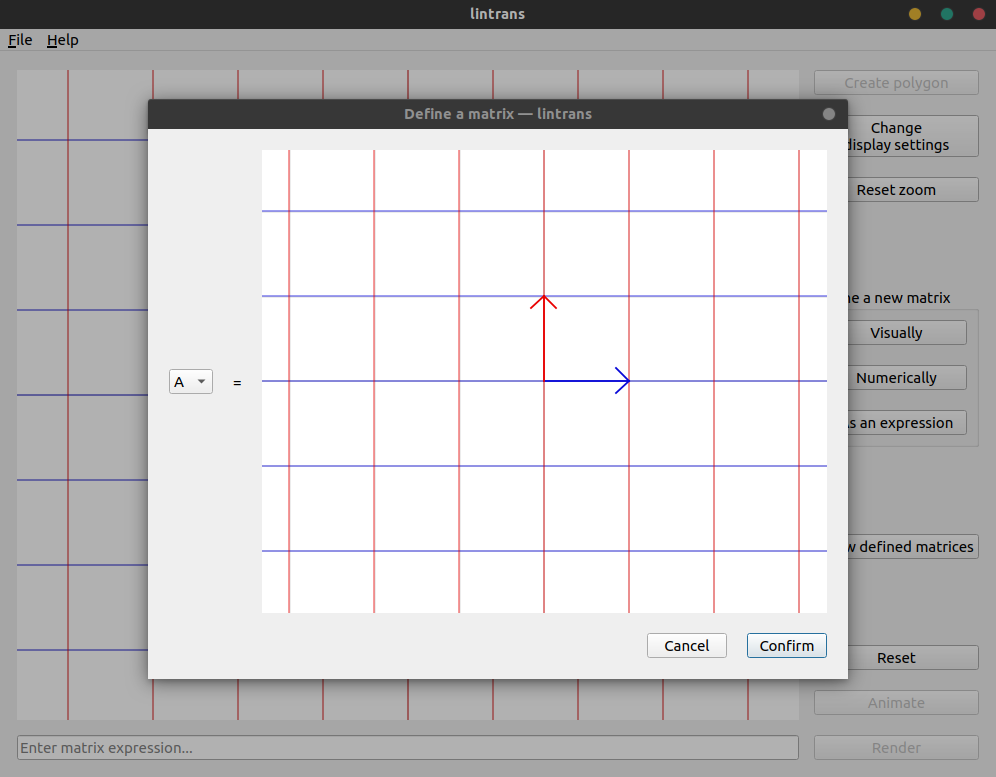
\includegraphics[width=0.95\linewidth]{evaluation/success-criteria/define-multiple-matrices/visual-dialog.png}
	\caption{The visual definition dialog}
	\label{fig:evaluation:success-criteria:define-multiple-matrices:visual-dialog.png}
\end{figure}

\subsubsection{Validating and parsing matrix expressions\label{evaluation:evaluating-success-criteria:validating-and-parsing-matrix-expressions}}

Criterion~\ref{success-criterion:validate-arbitrary-matrix-expressions} says that the program must be able to validate arbitrary matrix expressions and criterion~\ref{success-criterion:parse-matrix-expressions} says that it must be able to parse any valid expression. As shown in \S\ref{development:matrices-backend:rudimentary-parsing-and-evaluating}, \S\ref{development:matrices-backend:parsing-matrix-expressions}, and \S\ref{development:making-v0.2.2:parsing-parentheses}, the parser and validator are both complete and robust. I have fulfilled these success criteria.

\subsubsection{Rendering any valid expression\label{evaluation:evaluating-success-criteria:render-any-valid-expression}}

Criterion~\ref{success-criterion:render-any-valid-expression} says that the program must be able to render any valid matrix expression. Rendering is quite simple and I got it sorted early on in \S\ref{development:visualizing-matrices:implementing-basis-vectors} and \S\ref{development:visualizing-matrices:drawing-the-transformed-grid}. I have successfully fulfilled this criterion.

\subsubsection{Animating any valid expression\label{evaluation:evaluating-success-criteria:animate-any-valid-expression}}

Criterion~\ref{success-criterion:animate-any-valid-expression} says that the program must be able to animate from $\mathbf{I}$ to any valid expression. I expected animation to be difficult but it was surprisingly easy. I just had to draw multiple frames using a \texttt{for} loop. I have covered animation in \S\ref{development:visualizing-matrices:implementing-animation}, \S\ref{development:visualizing-matrices:preserving-determinants}, and \S\ref{development:making-v0.2.2:animating-rotations}. I have fulfilled this criterion.

\subsubsection{Applicative animation\label{evaluation:evaluating-success-criteria:applicative-animation}}

Criterion~\ref{success-criterion:applicative-animation} says that the program must be able to apply a matrix transformation to the current scene. This is essentially the crux of the app. I was initially inspired to create \texttt{lintrans} because I wanted a way to demonstrate the non-commutativity of matrix multiplication ($\mathbf{AB} \ne \mathbf{BA}$). For me, the best demonstration of this fact would be to show that applying two different matrices in different orders produces different results. Once I had the basis of an animation system, making it applicative wasn't as difficult as I expected.

I laid the groundwork for applicative animation in \S\ref{development:improving-the-gui:implementing-transitional-animation} and \S\ref{development:improving-the-gui:allowing-for-sequential-animation-with-commas} and then I implemented applicative animation by just allowing the user to change the display settings in \S\ref{development:adding-display-settings:creating-the-dataclass-and-implementing-applicative-animation}. I have fulfilled this criterion.

\subsubsection{Display matrix info\label{evaluation:evaluating-success-criteria:display-matrix-info}}

\fsbsr[0.4]{evaluation/success-criteria/display-matrix-info/dialog.png}{The display settings dialog}{ Criterion~\ref{success-criterion:display-matrix-info} says that the program should be able to display information about the currently displayed matrix. I added display settings in \S\ref{development:adding-display-settings} and these included things like determinants. I then polished determinant text in \S\ref{development:fixing-bugs-and-adding-polish:centering-text-in-the-determinant-parallelogram} and added eigenvectors and eigenlines in \S\ref{development:implementing-eigenstuffs}. I also added settings for animation timings in \S\ref{development:adding-display-settings:creating-the-dataclass-and-implementing-applicative-animation} and \S\ref{development:making-v0.2.2:adding-a-setting-for-animation-time}. \par I'm quite happy with these display settings. I think being able to change colours and label the basis vectors $i$ and $j$ would have been nice, but I got the important parts done. I have fulfilled this criterion.}

\begin{figure}[H]
	\centering
	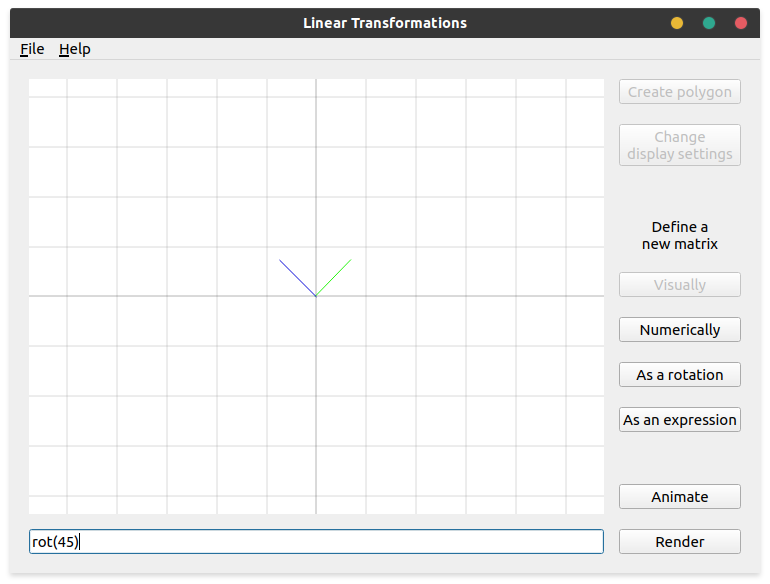
\includegraphics[width=0.95\linewidth]{evaluation/success-criteria/display-matrix-info/gui.png}
	\caption{A matrix being rendered with all the display settings on}
	\label{fig:evaluation:success-criteria:display-matrix-info:gui.png}
\end{figure}

\subsubsection{Saving and loading sessions\label{evaluation:evaluating-success-criteria:save-and-load-sessions}}

Criterion~\ref{success-criterion:save-and-load-sessions} says that the program should be able to save and load sessions. This was mostly a time restriction, but it shouldn't be particularly difficult to actually implement. I would create a dataclass to contain the data that we want to save, and use Python's \texttt{pickle} module to save it to a binary format for saving in a file. I failed to fulfil this criterion, mostly due to time.

\subsubsection{Transforming polygons\label{evaluation:evaluating-success-criteria:transform-polygons}}

Criterion~\ref{success-criterion:transform-polygons} says that the program should allow the user to define and transform an arbitrary polygon. I was unable to complete this criterion. I'm not entirely sure how I would've done it. Obviously I'd have a dialog to define a polygon, and that would probably use a list of coordinates, which it would return to the main window when the user confirmed the dialog. Then I would just transform each coordinate one-by-one and draw the before and after versions. I failed to complete this criterion, again mostly due to running out of time.

Overall, I completed 7 out of my 9 criteria. I wish I'd had time to get the polygons done, and maybe I should've focussed on that instead of fixing bugs. But I'm happy with \texttt{lintrans} as it is now. I will probably add these missing features in a future release.

\subsection{Assessing usability\label{evaluation:assessing-usability}}

The main usability features that I discussed in \S\ref{design:usability-features} were about colours, as well as layout and hotkeys.

The colours of the basis vectors are red and blue, as I said they should be. This allows users with common types of colour-blindness like deuteranopia to still distinguish parts of the UI. Refer to the images below to see that the colour scheme was a success\footnote{These images were generated using my fork of Color Oracle\cite{color-oracle-my-fork}.}:

\begin{figure}[H]
	\begin{minipage}{0.48\linewidth}
		\centering
		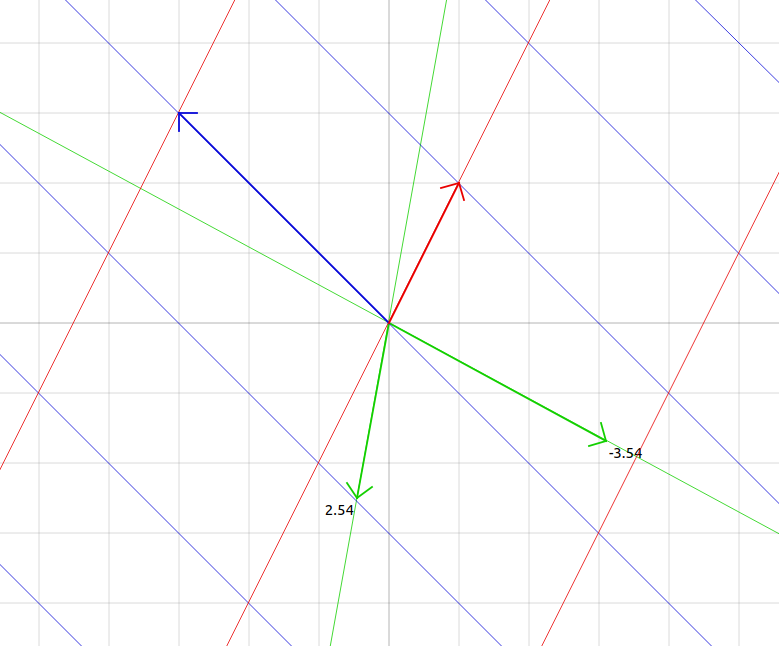
\includegraphics[width=\linewidth]{evaluation/usability/normal-vision.png}
		\caption{Normal vision}
		\label{fig:evaluation:usability:normal-vision.png}
	\end{minipage}\hfill
	\begin{minipage}{0.48\linewidth}
		\centering
		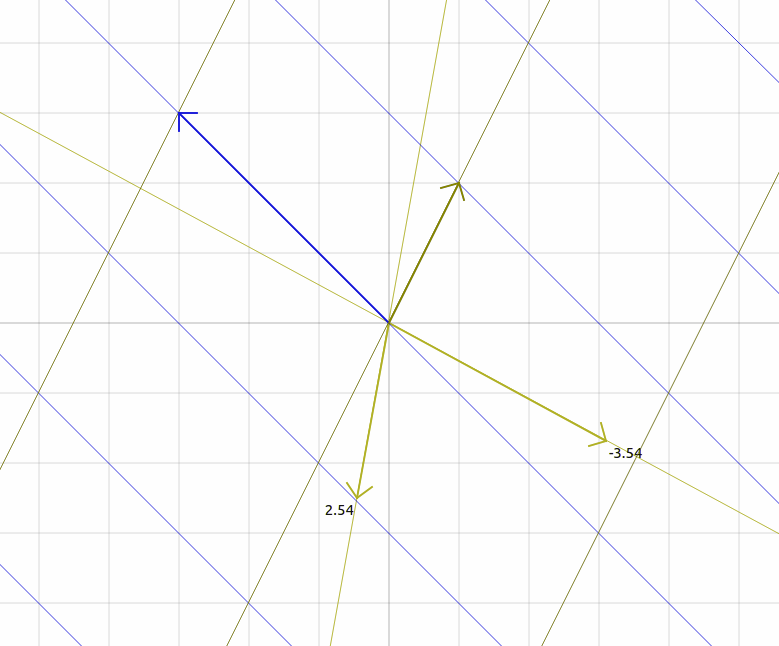
\includegraphics[width=\linewidth]{evaluation/usability/deuteranopia.png}
		\caption{Deuteranopia (common)}
		\label{fig:evaluation:usability:deuteranopia.png}
	\end{minipage}
\end{figure}
\begin{figure}[H]
	\begin{minipage}{0.48\linewidth}
		\centering
		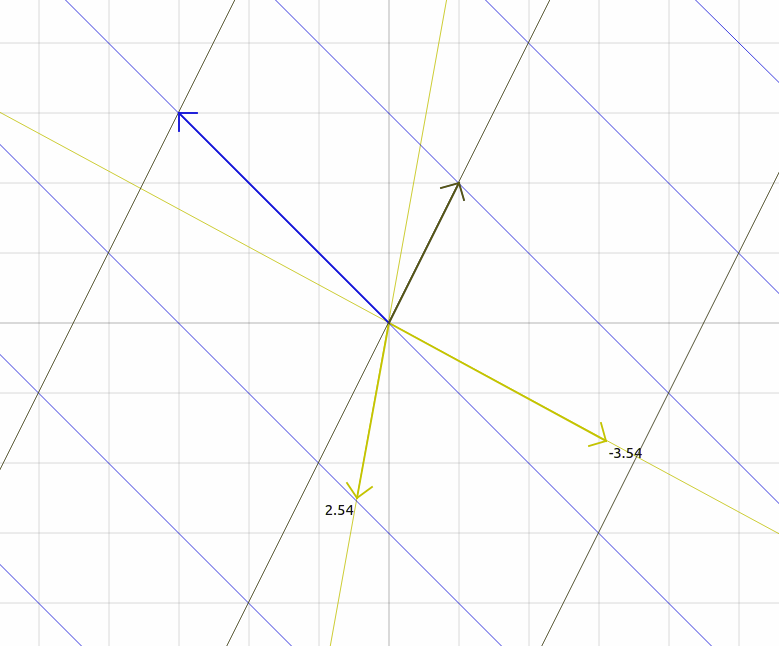
\includegraphics[width=\linewidth]{evaluation/usability/protanopia.png}
		\caption{Protanopia (rare)}
		\label{fig:evaluation:usability:protanopia.png}
	\end{minipage}\hfill
	\begin{minipage}{0.48\linewidth}
		\centering
		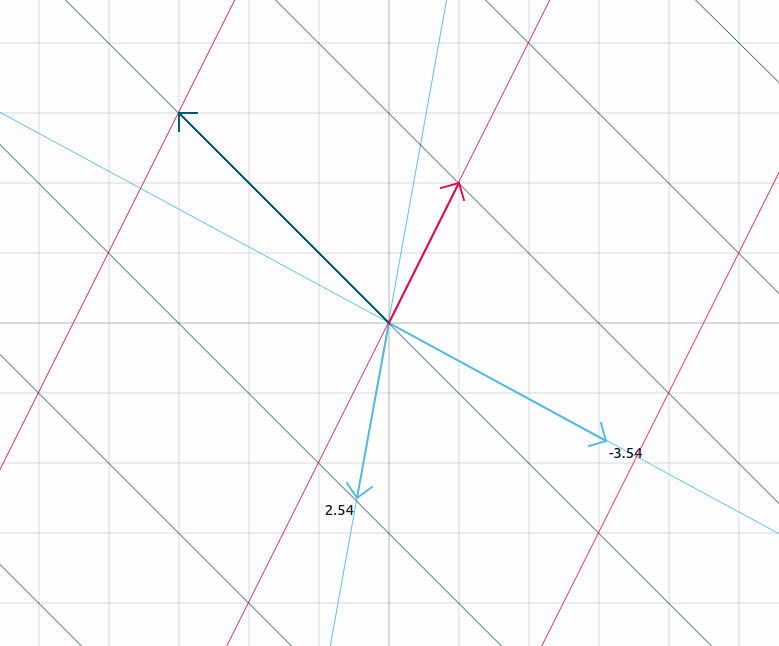
\includegraphics[width=\linewidth]{evaluation/usability/tritanopia.png}
		\caption{Tritanopia (very rare)}
		\label{fig:evaluation:usability:tritanopia.png}
	\end{minipage}
\end{figure}

My other usability features were consistent UI layouts and hotkeys. All dialogs follow the same pattern of having the confirm button in the bottom right corner with the cancel button to the left of it, which is consistent with common menu design. I consider this a success.

Most of the functionality in the app has associated hotkeys. Rendering, animating, resetting, opening dialogs, and toggling display settings all have dedicated hotkeys. I forgot to add a shortcut to open the info panel, but that change is tiny, so I can just do it right now:

%: 63f569328a1906976d725fa72da02e98e5d73afb
%: src/lintrans/gui/main_window.py:208-217 highlight=217

I would consider my use of hotkeys to be a success.

\subsection{Limitations\label{evaluation:limitations}}

\subsubsection{Feature completeness\label{evaluation:limitations:feature-completeness}}

As discussed in \S\ref{evaluation:evaluating-success-criteria:save-and-load-sessions} and \S\ref{evaluation:evaluating-success-criteria:transform-polygons}, \texttt{lintrans} is not feature complete according to my original success criteria. I attribute my failure to implement these features to me running out of time. If I focussed on implementing them instead of fixing bugs, then I definitely could've done them in time, but I wanted a more robust and bug-free app.

I think a more secure base allows for easier and more efficient expansion in the future. I can easily add these features in new versions, but I want to squash bugs early on so that I don't have to fix them later when the code base is larger. Overall, I wish I had more time to implement these missing features, but the core of the app is there, so I'll just add transforming arbitrary polygons and saving and loading sessions in the future.

\subsubsection{Distribution\label{evaluation:limitations:distribution}}

\texttt{lintrans} was surprisingly hard to distribute. I spend most of my time in the terminal, which makes it very easy to set up complete development environments and a virtual environment to manage the Python packages and interpreter needed to run \texttt{lintrans}. My stakeholders are teachers who don't even know what a shell is, let alone how to set up a virtual environment for Python. So I had to compile \texttt{lintrans} into a single Windows executable. That wasn't massively difficult, but it was certainly a headache. If I did this project again, I'd use a compiled language like Rust, Java, or C++, since those languages are much easier to distribute executables for.

Additionally, Rust can compile to WebAssembly\cite{compile-rust-to-wasm}, so I could make a web version of \texttt{lintrans}, which would avoid anyone having to download anything and would allow students to try it out very easily, perhaps even on their phones.

\subsection{Maintenance\label{evaluation:maintenance}}

\subsubsection{Class structure\label{evaluation:maintenance:class-structure}}

As you can see from the following internal import graph and class diagram, the class structure isn't fantastic.

\begin{figure}[H]
	\centering
	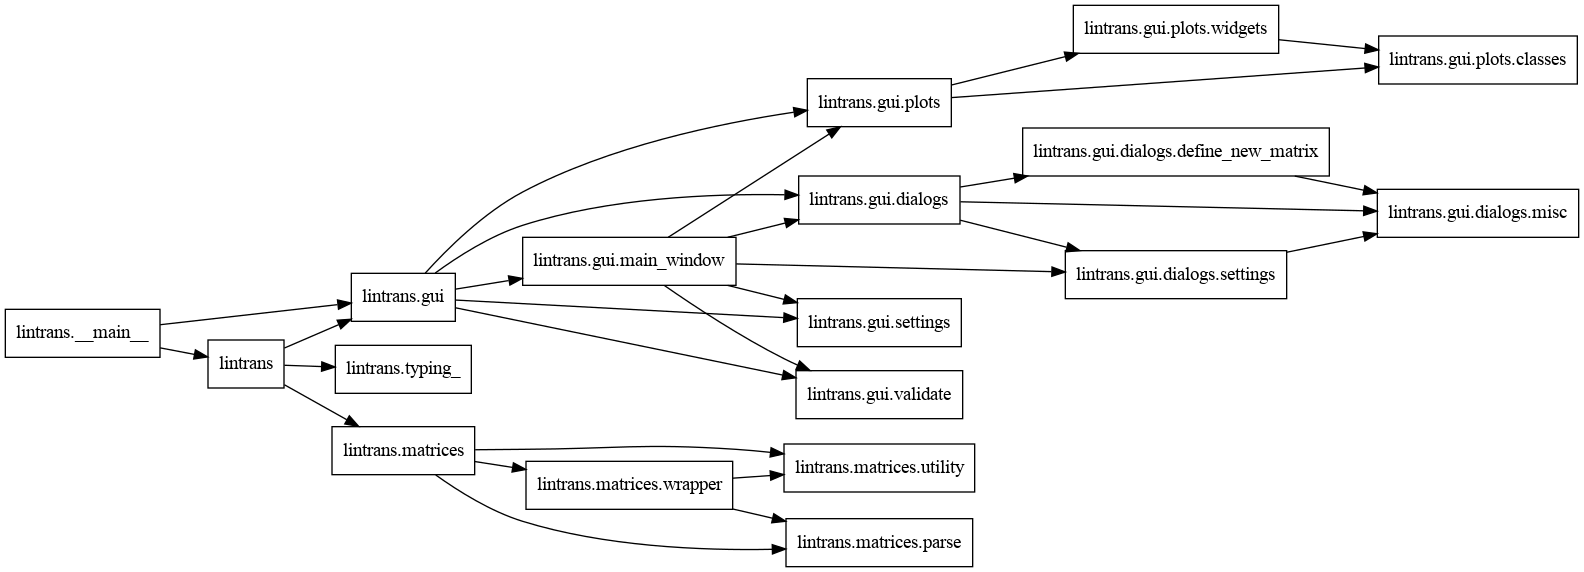
\includegraphics[width=0.95\linewidth]{evaluation/maintenance/int-imports.png}
	\caption{The final internal import graph}
	\label{fig:evaluation:maintenance:int-imports.png}
\end{figure}
\begin{figure}[H]
	\centering
	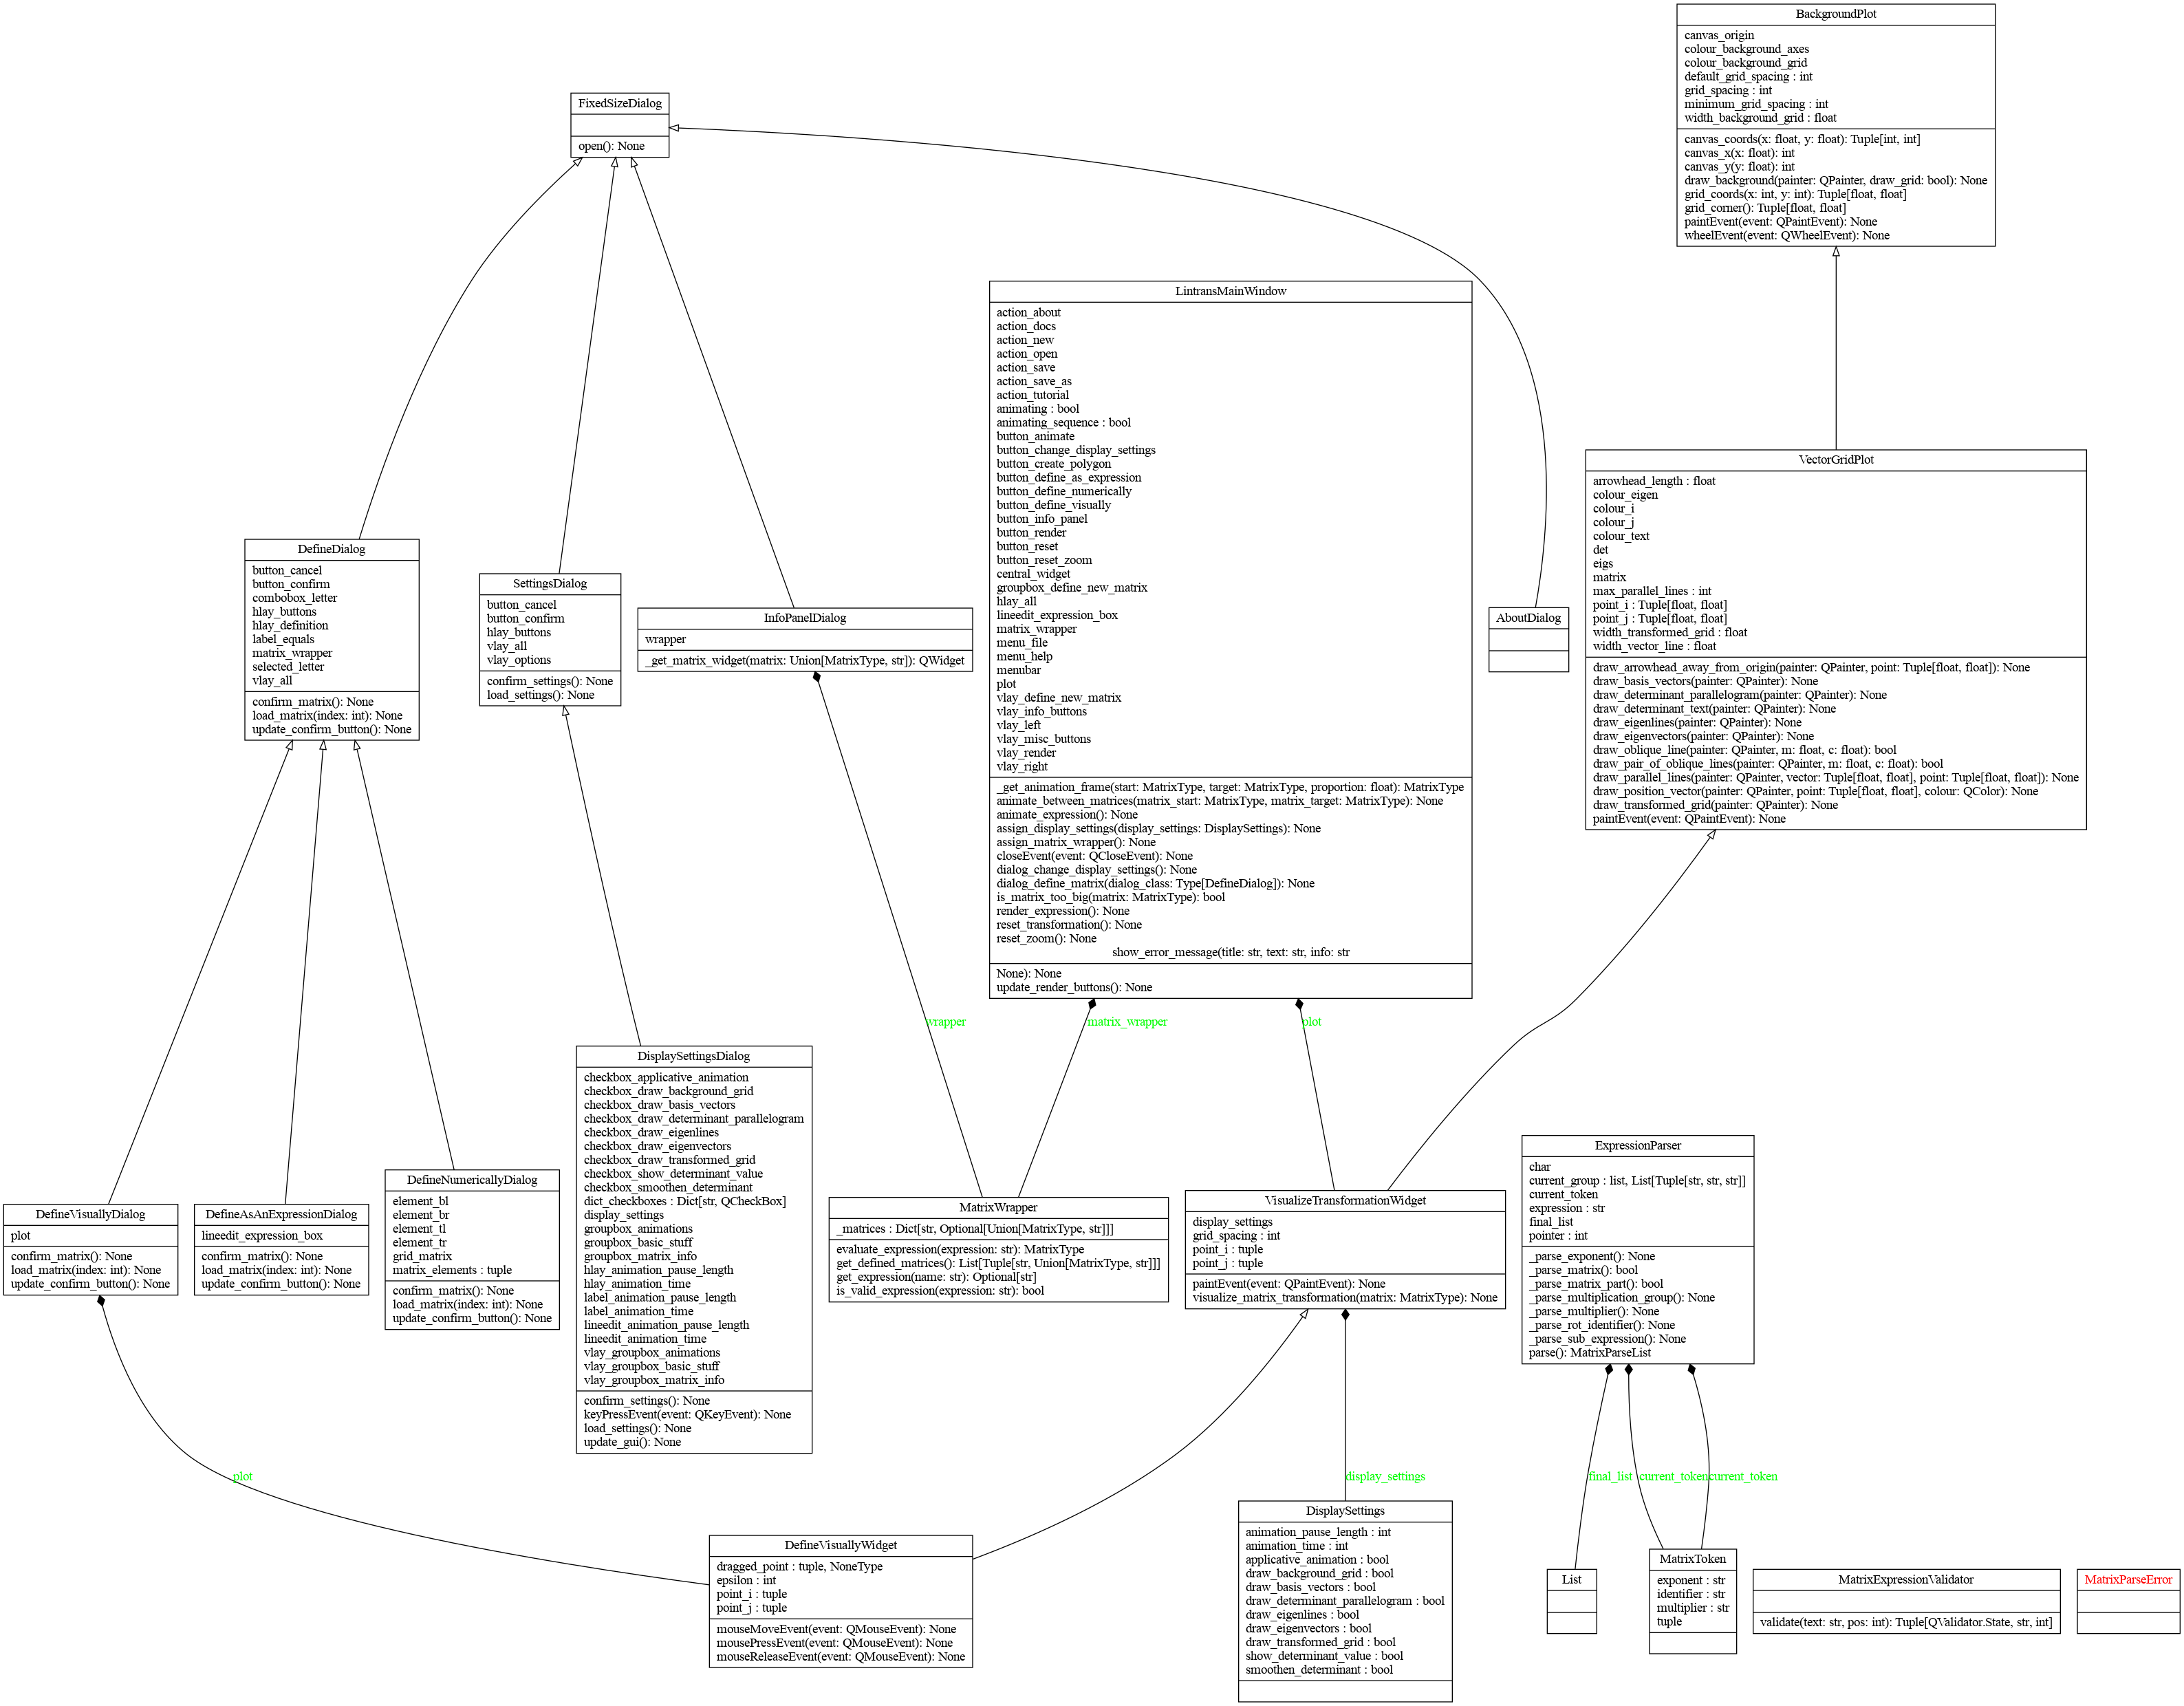
\includegraphics[width=0.95\linewidth]{evaluation/maintenance/classes.png}
	\caption{The final class diagram}
	\label{fig:evaluation:maintenance:classes.png}
\end{figure}

However, I believe that the classes are well named and in files which are equally well named. This makes maintaining them easier than you might suspect by looking at these diagrams. Additionally, all my variables and functions have sensible names which identify their purpose. Each class, method, and function is small and individual. The only \enquote{large} class is the main window, which makes sense because it has the most logic and is hard to split up.

Everything else is split into small enough logical chunks to make it pretty easy to maintain. I also have docstrings for every single class, method, and function, as well as comments to explain the complicated parts of algorithms. This annotation makes it much easier to remember what each thing does and how it does it.

Overall, there are a lot of classes and modules, but it's a complex program, so I think this is well justified. The logic is separate and modular.

\subsubsection{Type safety\label{evaluation:maintenance:type-safety}}

By far, my biggest maintainability problem is Python's lack of type safety. I use \texttt{mypy} to statically check the types of variables \textit{before} runtime, but the Python interpreter makes no real guarantees about what the types of variables will be \textit{at} runtime. This makes it much harder to debug things and introduces whole categories of bugs that would be impossible in a compiled, statically and strongly typed language like Rust, Java, or C++.

When I started \texttt{lintrans}, I didn't really care about types in a programming language and I was only really familiar with Python, so that's what I used. Since then, I've learned Rust and it's taught me the benefits of a static, strong type system. Rust doesn't even have \texttt{null} or exceptions. Python's \pyinline{None} and hidden exception throwing have caused several bugs already and will undoubtedly cause many more in the future. With Rust, these would be impossible, but in Python, they are seemingly hiding in every dark corner, just waiting to crash the program in some weird edge case.

I will need to stay on top of these types of bugs when maintaining \texttt{lintrans}, unless I decide to rewrite the whole thing in a compiled language.

\end{document}
